\documentclass[12pt,letterpaper]{article}
\usepackage{fullpage}
\usepackage[top=2cm, bottom=4.5cm, left=2.5cm, right=2.5cm]{geometry}
\usepackage{amsmath,amsthm,amsfonts,amssymb,amscd}
\usepackage{lastpage}
\usepackage{enumerate}
\usepackage{fancyhdr}
\usepackage{mathrsfs}
\usepackage{xcolor}
\usepackage{graphicx}
\usepackage{listings}
\usepackage{hyperref}

\hypersetup{%
  colorlinks=true,
  linkcolor=blue,
  linkbordercolor={0 0 1}
}

\renewcommand\lstlistingname{Algorithm}
\renewcommand\lstlistlistingname{Algorithms}
\def\lstlistingautorefname{Alg.}

\lstdefinestyle{Python}{
    language        = Python,
    frame           = lines,
    basicstyle      = \footnotesize,
    keywordstyle    = \color{blue},
    stringstyle     = \color{green},
    commentstyle    = \color{red}\ttfamily
}

\setlength{\parindent}{0.0in}
\setlength{\parskip}{0.05in}

% Edit these as appropriate
\newcommand\course{Machine Learning}
\newcommand\hwnumber{1}                  % <-- homework number
\newcommand\NetIDa{WangZhiyi, 922182514} % <-- NetID of person #1
\newcommand\NetIDb{ZhangTianyao, 922182332} % <-- NetID of person #2 (Comment this line out for problem sets)

\pagestyle{fancyplain}
\headheight 35pt
\lhead{\NetIDa}
\lhead{\NetIDa\\\NetIDb}                 % <-- Comment this line out for problem sets (make sure you are person #1)
\chead{\textbf{\Large Homework \hwnumber}}
\rhead{\course \\ \today}
\lfoot{}
\cfoot{}
\rfoot{\small\thepage}
\headsep 1.5em

\begin{document}

\section*{Problem 1}
As the prisoner cannot remember his former choice,he faces the same situation when he makes choice. Assume expected time to get free is $E(t)$ which is composed by three situations, he chooses the tunnel leads to freedom within 3 hours, others two are lead to freedom within $7+E(t)$ or $5+E(t)$. Each of them has a probability of $\frac{1}{3}$. Therefore, the $E(t)$ is calculated by equation\ref{eq1}
\begin{equation}\label{eq1}
E\left( t \right) =\frac{1}{3}\cdot 3+\frac{1}{3}\cdot \left[ E\left( t \right) +5 \right] +\frac{1}{3}\cdot \left[ E\left( t \right) +7 \right]
\end{equation}
Solve equation \ref{eq1}the expected time it will take the prisoner to obtain freedom is 15 hours.
\section*{Problem 2}
\subsection*{Question a}
{\bf Model:} $i.d.d$ samples $\left\{ x_i \right\} _{i=1}^{n}$ are normally distributed, $p\left( x|y \right) \sim \mathcal{N}\left( y,1 \right)$\\
{\bf Parameter:} $y$ is the mean of the distribution.\\
{\bf Goal:} Get the $y$ when samples are given, which leads the samples have the max probability to happen.\\
{\bf Probability density of $X$} is calculated by equation \ref{eq2}
\begin{equation}\label{eq2}
  p\left( X=x_i|y=\hat{y}_{MLE} \right) =\frac{1}{\sqrt{2\pi \sigma ^2}}e^{-\frac{\left( x_i-\hat{y}_{MLE} \right) ^2}{2\sigma ^2}}
\end{equation}

{\bf Likelihood Function} is given by equation
\begin{eqnarray}\label{eq3}
% \nonumber % Remove numbering (before each equation)
  L\left( \hat{y}_{MLE} \right) &=& \prod_{i=1}^n{p\left( X=x_i|y=\hat{y}_{MLE} \right)}\\
  &=& \prod_{i=1}^n{\frac{1}{\sqrt{2\pi}}e^{-\frac{( x_i-\hat{y}_{MLE} ) ^2}{2}}} \nonumber \\
  &=& \frac{n}{\sqrt{2\pi^2}}e^{-\frac{1}{2}\sum_{i=1}^n{\left( x_i-\hat{y}_{MLE} \right) ^2}} \nonumber
\end{eqnarray}

Then use $ln$ function to simplify,
\begin{eqnarray}\label{eq4}
% \nonumber % Remove numbering (before each equation)
  \ln(L(\hat{y}_{MLE})) &=& \ln \left( \frac{n}{\sqrt{2\pi}} \right) -\frac{1}{2}\sum_{i=1}^n{\left( x_i-\hat{y}_{MLE} \right) ^2}
\end{eqnarray}
Derivative,

\begin{eqnarray}\label{5}
% \nonumber % Remove numbering (before each equation)
\frac{d\ln \left( L\left( \hat{y}_{MLE} \right) \right)}{d\hat{y}_{MLE}}&=&\frac{1}{2}\sum_{i=1}^n{\left( x_i-\hat{y}_{MLE} \right)}
\end{eqnarray}
Set the derivative equal to 0. We can get $\hat{y}_{MLE}$
\begin{equation}\label{eq6}
  \hat{y}_{MLE}=\frac{1}{n}\sum_{i=1}^n{x_i}
\end{equation}
\subsection*{Question b}

{\bf MAP function:} Use the $\hat{y}_{MLE}$ in equation\ref{eq3} to
\begin{eqnarray}\label{eq7}
  M\left( \hat{y} \right) &=& p\left( \hat{y} \right) \cdot L\left( \hat{y}_{MLE} \right)\\ \nonumber
  &=& \frac{\sqrt{s}}{\sqrt{2\pi}}e^{-\frac{s\left( \hat{y}-z \right) ^2}{2}}\cdot \frac{n}{\sqrt{2\pi}}e^{-\frac{1}{2}\sum_{i=1}^n{\left( x_i-\hat{y}\right) ^2}}
\end{eqnarray}
Use $\ln(x)$ function to simplify:
\begin{equation}\label{eq8}
   L(\hat{y})=\ln \left( \frac{\sqrt{s}}{\sqrt{2\pi}} \right) -\frac{s\left( \hat{y}-z \right) ^2}{2}+\ln \left( \frac{n}{\sqrt{2\pi}} \right) -\frac{1}{2}\sum_{i=1}^n{\left( x_i-\hat{y} \right) ^2}
\end{equation}
Set $\frac{dL\left( y \right)}{dy}$ equals to 0 to get the $\underset{\hat{y}\in R}{arg\,\,\max}L\left( y \right) $
\begin{equation}\label{eq9}
  \frac{dL\left( \hat{y} \right)}{d\hat{y}}=-s\left( \hat{y}-z \right) +\sum_{i=1}^n{\left( x_i-\hat{y} \right)}=0
\end{equation}
Solve equation\ref{eq9} then get the $\hat{y}_{1}$
\begin{equation}\label{eq10}
  \hat{y}_1=\frac{n}{n+s}\hat{y}_{MLE}+\frac{sz}{n+s}
\end{equation}

\subsection*{Question c}
The density function of $y$ is
\begin{equation}\label{eq11}
  p\left( y \right) =\begin{cases}
	\frac{1}{2},-1\leqslant y\leqslant 1\\
	\text{0,}o.w\\
\end{cases}
\end{equation}

{\bf MAP function}
\begin{eqnarray}\label{eq12}
M\left( \hat{y} \right)
&=& p\left( \hat{y} \right) \cdot L\left( \hat{y}_{MLE} \right)\\ \nonumber
&=& \frac{1}{2}\cdot \frac{n}{\sqrt{2\pi}}e^{-\frac{1}{2}\sum_{i=1}^n{\left( x_i-\hat{y}\right) ^2}}
\end{eqnarray}

Use $\ln$ function to simplify:
\begin{equation}\label{eq13}
  L(\hat{y})=\ln[ M(\hat{y})]=\ln(\frac{1}{2})+\ln(\frac{n}{\sqrt{2\pi}})-\frac{1}{2}\sum_{i=1}^n{\left( x_i-\hat{y} \right) ^2}
\end{equation}
Set $\frac{dL\left( y \right)}{dy}$ equals to 0 to get the $\underset{\hat{y}\in R}{arg\,\,\max}L\left( y \right) $ when $-1\leqslant y_{MLE}\leqslant 1$, namely
\begin{equation}\label{eq14}
  \frac{dL\left( y \right)}{dy}=\sum_{i=1}^n{\left( x_i-\hat{y} \right)}=0
\end{equation}
Solve equation\ref{eq14}, we can get $\hat{y}_2=y_{MLE}$ when $-1\leqslant y_{MLE}\leqslant 1$, while when $y_{MLE}<-1$, $\hat{y}_2=-1$, when $y_{MLE}>1$, $\hat{y}_2=1$, therefore
\begin{equation}\label{eq15}
  \hat{y}_2=\begin{cases}
	-\text{1, }y_{MLE}<-1\\
	y_{MLE}, -1\leqslant y_{MLE}\leqslant 1\\
	\text{1,}y_{MLE}>1\\
\end{cases}
\end{equation}


%Answer to the problem goes here.
%
%\begin{enumerate}
%  \item
%   Problem 1 part 1 answer here.
%  \item
%    Problem 1 part 2 answer here.
%
%    Here is an example typesetting mathematics in \LaTeX
%\begin{equation*}
%    X(m,n) = \left\{\begin{array}{lr}
%        x(n), & \text{for } 0\leq n\leq 1\\
%        \frac{x(n-1)}{2}, & \text{for } 0\leq n\leq 1\\
%        \log_2 \left\lceil n \right\rceil \qquad & \text{for } 0\leq n\leq 1
%        \end{array}\right\} = xy
%\end{equation*}
%
%    \item Problem 1 part 3 answer here.
%
%    Here is an example of how you can typeset algorithms.
%    There are many packages to do this in \LaTeX.
%
%    \lstset{caption={Caption for code}}
%    \lstset{label={lst:alg1}}
%    \begin{lstlisting}[style = Python]
%    from package import Class # Mesh required for..
%
%    cinstance = Class.from_obj('class.obj')
%    cinstance.go()
%    \end{lstlisting}
%
%  \item Problem 1 part 4 answer here.
%
%    Here is an example of how you can insert a figure.
%    \begin{figure}[!h]
%    \centering
%    
\includegraphics[width=0.3\linewidth]{heidi.jpg}
%    \caption{Heidi attacked by a string.}
%    \end{figure}
%\end{enumerate}



\section{Problem 3}
\subsection*{Question a}
Random variables of Poisson distribution:
\begin{equation}\label{3aeq1}
  P(X=k)=\frac{\lambda^k}{k!}e^{-\lambda}
\end{equation}

a set of iid samples $D=\{x_1,x_2,\cdots,x_N\}$ drawn according to the Poisson probability mass:
\begin{equation}\label{3aeq2}
  L(\lambda)=P(x_1,x_2,\cdots,x_N)=P(x_1)P(x_2)\cdots P(x_N)
\end{equation}
We use $\ln$ to simplify
\begin{eqnarray}\label{3aeq3}
% \nonumber % Remove numbering (before each equation)
lnL(\lambda)
&=&lnP(x_1)+lnP(x_2)+\cdots+lnP(x_N)\\
&=&\sum^N_{i=1}(x_iln\lambda-\sum^{x_i}_{j=1}lnj-\lambda)\nonumber
\end{eqnarray}
ML condition tells:

\begin{equation}\label{3aeq4}
\frac{\partial lnL(\lambda)}{\partial\lambda}=\sum^N_{i=1}\frac{x_i}\lambda-N=0\\
\therefore \lambda_{ML}=\frac1N\sum^N_{i=1}x_i
\end{equation}
\begin{eqnarray}\label{3aeq5}
  E(\hat{\lambda})
  &=&E(\frac1N\sum^N_{i=1}x_i|\lambda)\\
  &=&\frac1N\sum^N_{i=1}E(x_i|\lambda)\nonumber\\
  &=&\frac1N\sum^N_{i=1}\lambda\nonumber\\\
  &=&\lambda\nonumber
\end{eqnarray}
note that $E[X]=\lambda$:
\begin{eqnarray}
% \nonumber % Remove numbering (before each equation)
  E(\hat{x_k})
  &=&  \sum^\infty_{i=1}x_i\frac{\lambda^{x_i}}{x_i!}e^{-\lambda} \nonumber\\
  &=& \lambda\sum^\infty_{i=0}\frac{\lambda^{x_i}}{x_i!}e^{-\lambda}\nonumber
\end{eqnarray}
So the MLE is not biased.


\subsection*{Question b}
Use $y$ and $k$ to reexpress $\lambda$:
\begin{equation}
  y=P(X=0)^2=e^{-2\lambda}
\end{equation}
So $\lambda=-\frac12lny$. Then replace $\lambda$ into the formula.
\begin{equation}
  P(X=k)=\frac{\lambda^k}{k!}e^{-\lambda}=\frac{(-\frac12lny)^k}{k!}\sqrt{y}
\end{equation}
to a single $k$, here is maximum likelihood estimator:
\begin{equation}
  \hat{y}_{MLE}=\underset{y}{arg\,\max}P(X=k)=\frac1n\sum^n_{i=1}x_i
\end{equation}
Because $n=1$, $\hat{y}_{MLE}=e^{-2\lambda}$
\begin{equation}
  b(y)=E(y)-\hat{y}_{MLE}=\sum^\infty_{k=0}e^{-2k}\frac{\lambda^k}{k!}e^{-lambda}=e^{e^{-2}\lambda-\lambda}-e^{-2\lambda}\neq{0}
\end{equation}
Obviously, $\hat y_{MLE}$ is biased.
\subsection*{Question c}
Assume that $y_U$ is biased:
\begin{equation}
  E(y_{MLE})=\sum^\infty_{k=0}y_UP(X=k)=\sum^\infty_{k=0}y_U\frac{\lambda^k}{k!}e^{-\lambda}=y=e^{-2\lambda}
\end{equation}
Because $e^\lambda=\sum^\infty_{k=0}\frac{\lambda^k}{k!}$,$y_U=(-1)^k$
\subsection*{Question d}

\begin{eqnarray}
% \nonumber % Remove numbering (before each equation)
MSE_{ML}
&=&E\left[ \left( p_{MLE}-p \right) ^2 \right]\\
&=&\sum_{k=1}^{\infty}{\left( e^{-2k}-e^{-2\lambda} \right)}^2\frac{\lambda ^k}{k!}e^{-\lambda}
\nonumber\\
&=&e^{\left( e^{-4}-1 \right) \lambda}-2e^{\left( e^{-2}-2 \right) \lambda}+e^{-4\lambda}MSE_U
\nonumber\\
&=&E\left[ \left( p_U-p \right) ^2 \right]
\nonumber\\
&=&\sum_{k=1}^{\infty}{\left( \left( -1 \right) ^k-e^{-2\lambda} \right)}^2\frac{\lambda ^k}{k!}e^{-\lambda}
\nonumber\\
&=&1-e^{-4\lambda}\nonumber
\end{eqnarray}

calculate it with Python, set:
\begin{eqnarray}
% \nonumber % Remove numbering (before each equation)
  f(x)
  &=&MSE_{ML}-MSE_U \\
  &=&[e^{(e^{-4}-1)x}-2e^{(e^{-2}-2)x}+e^{-4x}]-[1-e^{-4x}],x>0 \nonumber
\end{eqnarray}

\begin{lstlisting}[style = Python]
import matplotlib.pyplot as plt
import numpy as np
import math

e = math.e

x = np.linspace(0, 20, 500)
y = (e**((e**(-4)-1)*x) - 2*e**((e**(-2)-2)*x) + e**(-4*x)) - (1 - e**(-4*x))

plt.title("compare(ML vs U)")
plt.plot(x, y)
plt.show()
\end{lstlisting}

and then draw the image of $f(x)$, it shows in figure\ref{fg1}
\begin{figure}
  \centering
  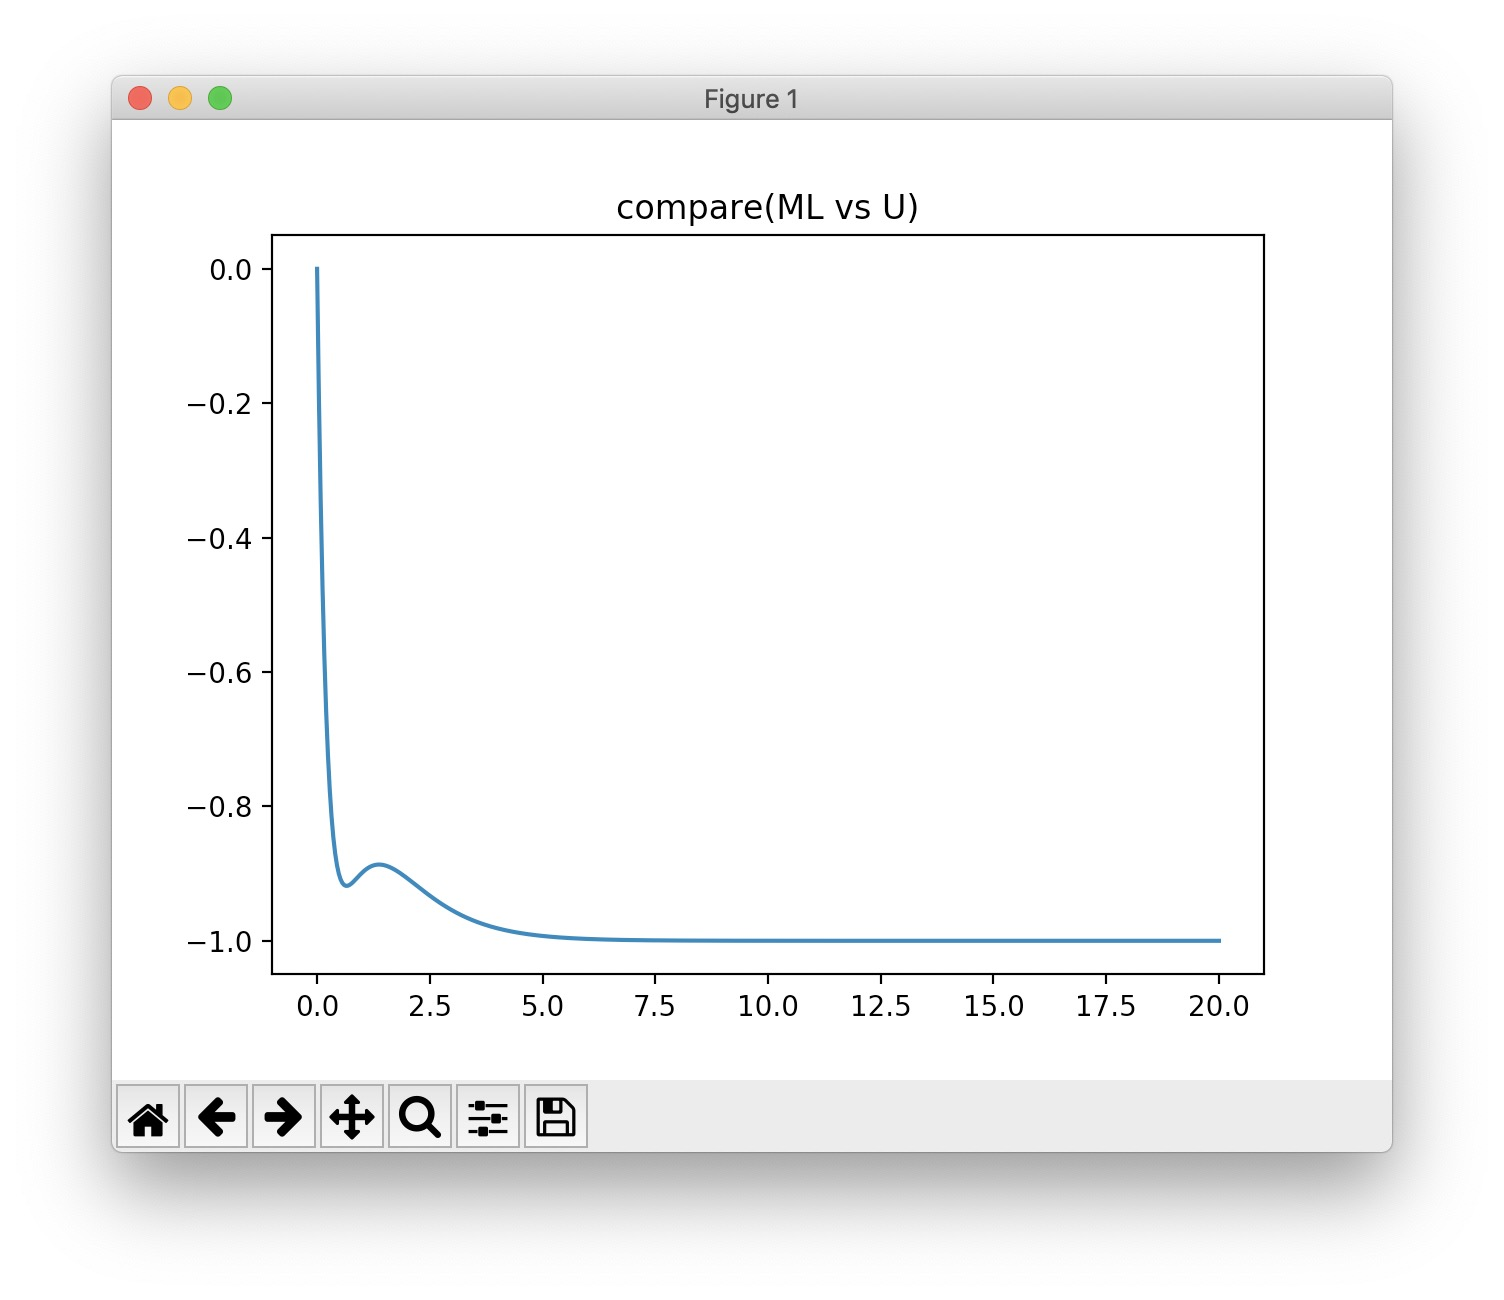
\includegraphics[width=10cm]{001.jpg}
  \caption{Figure1}\label{fg1}
\end{figure}


$f(x)<0,x>0$
$\therefore MSE_{ML}<MSE_U$



\section*{Problem 4}
\subsection*{Question a}

\begin{equation}
  \hat\mu=\frac1n\sum^n_{i=1}x_i
\end{equation}
\begin{equation}
  \hat\Sigma=\frac1n\sum^n_{i=1}(x_i-\hat\mu)(x_i-\hat\mu)^T
\end{equation}

\begin{scriptsize}
\begin{eqnarray}
% \nonumber % Remove numbering (before each equation)
E\left[ \hat{\Sigma}_{MLE} \right]
&=&E\left[ \frac{1}{n}\sum_{i=1}^n{\left( x_i-\hat{\mu}_{MLE} \right)}\left( x_i-\hat{\mu}_{MLE} \right) ^T \right]
\\
&=&\frac{1}{n}\sum_{i=1}^n{E}\left[ x_i\cdot x_{i}^{T}-x_i\cdot \hat{\mu}_{MLE}^{T}-\hat{\mu}_{MLE}\cdot x_{i}^{T}+\hat{\mu}_{MLE}\cdot \hat{\mu}_{MLE}^{T} \right]
\nonumber\\
&=&\frac{1}{n}\sum_{i=1}^n{E}\left[ x_i\cdot x_{i}^{T}-x_i\cdot \frac{1}{n}\sum_{j=1}^n{x}_{j}^{T}-\frac{1}{n}\sum_{j=1}^n{x}_j\cdot x_{i}^{T}+\frac{1}{n}\sum_{j=1}^n{x}_j\cdot \frac{1}{n}\sum_{j=1}^n{x}_{j}^{T} \right]
\nonumber\\
&=&\frac{1}{n}\sum_{i=1}^n{\left( E\left[ x_i\cdot x_{i}^{T} \right] -\frac{2}{n}\sum_{j=\text{1,}j\ne i}^n{E}\left[ x_i\cdot x_{j}^{T} \right] -\frac{2}{n}E\left[ x_i\cdot x_{i}^{T} \right] +\frac{1}{n^2}\sum_{j=i}{E}\left[ x_j\cdot x_{j}^{T} \right] +\frac{1}{n^2}\sum_{j=1}^n{\sum_{k=\text{1,}k\ne j}^n{E}}\left[ x_j\cdot x_{k}^{T} \right] \right)}
\nonumber\\
&=&\frac{1}{n}\sum_{i=1}^n{\left( \frac{n-2}{n}E\left[ x_i\cdot x_{i}^{T} \right] -\frac{2n-2}{n}\mu _{MLE}\cdot \mu _{MLE}+\frac{1}{n}E\left[ x_i\cdot x_{i}^{T} \right] +\frac{n^2-n}{n^2}\mu _{MLE}\cdot \mu _{MLE}^{T} \right)}
\nonumber\\
&=&\frac{n-1}{n^2}\sum_{i=1}^n{E}\left[ x\cdot x^T-x\cdot \mu ^T-\mu \cdot x^T+\mu \cdot \mu ^T \right]
\nonumber\\
&=&\frac{n-1}{n^2}\sum_{i=1}^n{E}\left[ \left( x-\mu \right) \left( x-\mu \right) ^T \right]
\nonumber\\
&=&\frac{n-1}{n^2}\sum_{i=1}^n{\Sigma}
\nonumber\\
&=&\frac{n-1}{n}\Sigma\nonumber 
\end{eqnarray}
\end{scriptsize}
Obviously, $\hat\Sigma_{MLE}$ is biased

\subsection*{Question b}
\begin{equation}
  \hat\Sigma'=\frac{n}{n-1}\hat\Sigma_{MLE}=\frac1{n-1}\sum^n_{i=1}(x_i-\hat\mu)(x_i-\hat\mu)^T
\end{equation}


\section*{Problem 5}
\subsection*{Question a}
We choose $k$ samples from range $\left[ \text{1,2,}\cdots ,N \right]$So the {\bf ML Function}is
\begin{equation}\label{5aeq1}
  M(N)=p\left( x_1,x_2,\cdots ,x_k|N \right) =\prod_{i=0}^{i=k-1}{\frac{1}{N-i}}
\end{equation}
When we get the $\underset{N\in R}{arg\,\,\max}M\left( N \right)$
Then define a new function $t(N)$ to simplify, we just need to consider about denominator of $M(x)$
\begin{equation}\label{5aeq2}
  t\left( N \right) =N\cdot \left( N-1 \right) \cdots \left( N-k+1 \right) =\frac{N!}{k!\left( N-k \right) !}\cdot k!=C_{N}^{k}\cdot k!
\end{equation}
It is easy to find that $\underset{N\in R}{arg\,\,\max}M\left( N \right)=\underset{N\in R}{arg\,\,\min}t\left( N \right)$
Then we find the $\underset{N\in R}{arg\,\,\min}t\left( N\right)$
\begin{eqnarray}\label{5aeq3}
  \underset{N\in R}{arg\,\,\min}t\left( N \right)
  &=& \underset{N\in R}{arg\,\,\min}\,\,C_{N}^{k}\cdot k! \\
  &=& \underset{N\in R}{arg\,\,\min}\,\,\frac{N!}{k!\left( N-k \right) !} \nonumber \nonumber \\
  &=& \underset{N\in R}{arg\,\,\min}N \nonumber \\
  &=& \underset{x\in \left\{ x_i \right\} _{1}^{k}}{arg\,\,\max}x_i \nonumber
\end{eqnarray}
Therefore, $\hat{N}_{MLE}=max\{x_i|x_i\in \{ x_i \} _{1}^{k}\}$
\subsection*{Question b}
We should prove $E(\hat{N}_{MLE})\ne N$

\begin{scriptsize}
\begin{eqnarray}\label{5beq1}
% \nonumber % Remove numbering (before each equation)
  E(\hat{N}_{MLE})
   &=& \sum_{i=1}^N{P\left( \hat{N}_{MLE}=i \right) \cdot i}  \\
   &=& \sum_{i=1}^N{\left[ P\left( \hat{N}_{MLE}\leqslant i \right) -P\left( \hat{N}_{MLE}\leqslant i-1 \right) \right] \cdot i}\nonumber \nonumber \\
   &=& \underset{i\leqslant k}{\underbrace{\left( \frac{C_{k}^{k}}{C_{N}^{k}}-0 \right) \cdot k}}+\underset{k+1\leqslant i\leqslant N}{\underbrace{\sum_{i=k+1}^N{\left[ \frac{C_{i}^{k}}{C_{N}^{k}}-\frac{C_{i-1}^{k}}{C_{N}^{k}} \right] \cdot i}}}+\underset{i=N+1}{\underbrace{\left( 1-\frac{C_{N}^{k}}{C_{N}^{k}} \right) }}+\underset{i>N+1}{\underbrace{\left( 1-1 \right) }} \nonumber \\
   %%%%%%%%%%%%%%%%%%%%%%%%%%%%%%
   &=& \frac{k}{\frac{N!}{k!\left( N-k \right) !}}+\sum_{i=k+1}^N{\left[ \frac{\frac{i!}{k!\left( i-k \right) !}}{\frac{N!}{k!\left( N-k \right) !}}-\frac{\frac{\left( i-1 \right) !}{k!\left( i-k-1 \right) !}}{\frac{N!}{k!\left( N-k \right) !}} \right] \cdot i}\nonumber \\
   &=& \frac{k\cdot k!\left( N-k \right) !}{N!}+\sum_{i=k+1}^N{\left[ \frac{i!\left( N-k \right) !}{\left( i-k \right) !N!}-\frac{\left( i-1 \right) !\left( N-k \right) !}{\left( i-k-1 \right) !N!} \right] \cdot i} \nonumber\\
   &=& \frac{k\cdot k!\left( N-k \right) !}{N!}+\frac{\left( N-k \right) !}{N!}\cdot \sum_{i=k+1}^N{\left[ \frac{i!}{\left( i-k \right) !}+\frac{\left( i-1 \right) !}{\left( i-k-1 \right) \text{!}} \right] \cdot i} \nonumber\\
   &=& \frac{\left( N-k \right) !}{N!}\left( k\cdot k!+\sum_{i=k+1}^N{\left[ \frac{i!}{\left( i-k \right) !}+\frac{i!}{\left( i-k \right) \text{!}}\cdot \frac{i-k}{i} \right] \cdot i} \right)\nonumber\\
   &=& \frac{\left( N-k \right) !}{N!}\left( k\cdot k!+\sum_{i=k+1}^N{\frac{i!}{\left( i-k \right) !}\left( 2i-k \right)} \right)\nonumber\\
   &=& \frac{\left( N-k \right) !}{N!}\left( k\cdot k!+\left( k+1 \right) !\sum_{i=k+1}^N{\frac{i!}{\left( i-k-1 \right) !\left( k+1 \right) !}\cdot \frac{2i-k}{i-k}} \right)\nonumber\\
   &=& \frac{\left( N-k \right) !}{N!}\left( k\cdot k!+\left( k+1 \right) !\sum_{i=k+1}^N{\frac{i!}{\left( i-k-1 \right) !\left( k+1 \right) !}\cdot \left( 1+\frac{i}{i-k} \right)} \right)\nonumber\\
   &=& \frac{\left( N-k \right) !}{N!}\left( k\cdot k!+\left( k+1 \right) !\cdot \left( \sum_{i=k+1}^N{\frac{i!}{\left( i-k-1 \right) !\left( k+1 \right) !}}+\sum_{i=k+1}^N{\frac{i!}{\left( i-k-1 \right) !\left( k+1 \right) !}\cdot \frac{i}{i-k}} \right) \right)\nonumber\\
   &=& \frac{\left( N-k \right) !}{N!}\left( k\cdot k!+\left( k+1 \right) !\cdot \left( \sum_{i=k+1}^N{\frac{i!}{\left( i-k-1 \right) !\left( k+1 \right) !}}+\sum_{i=k+1}^N{\frac{i!}{\left( i-k-1 \right) !\left( k+1 \right) !}\cdot \frac{i}{i-k}} \right) \right)\nonumber\\
   &=& \frac{\left( N-k \right) !}{N!}\left( k\cdot k!+\left( k+1 \right) !\cdot \left( \frac{\left( N+1 \right) !}{\left( N-k+1 \right) !\left( k+1+1 \right) !}+\sum_{i=k+1}^N{\frac{i!}{\left( i-k-1 \right) !\left( k+1 \right) !}\cdot \left( 1+\frac{k}{i-k} \right)} \right) \right)\nonumber\\
   &=& \frac{\left( N-k \right) !}{N!}\left( k\cdot k!+\left( k+1 \right) !\cdot \left( \frac{2\left( N+1 \right) !}{\left( N-k+1 \right) !\left( k+1+1 \right) !}+\sum_{i=k+1}^N{\frac{i!}{\left( i-k \right) !\left( k+1 \right) !}\cdot k} \right) \right)\nonumber\\
   &=& \frac{\left( N-k \right) !}{N!}\left( k\cdot k!+\left( k+1 \right) !\cdot \left( \frac{2\left( N+1 \right) !}{\left( N-k+1 \right) !\left( k+1+1 \right) !}+\frac{k}{\left( k+1 \right)}\cdot \left( \sum_{i=k}^N{\frac{i!}{\left( i-k \right) !k!}}-1 \right) \right) \right)\nonumber\\
   &=& \frac{\left( N-k \right) !}{N!}\left( k\cdot k!+\left( k+1 \right) !\cdot \left( \frac{2\left( N+1 \right) !}{\left( N-k+1 \right) !\left( k+1+1 \right) !}+\frac{k}{\left( k+1 \right)}\cdot \left( \frac{\left( N+1 \right) !}{\left( N-k \right) !\left( k+1 \right) !}-1 \right) \right) \right)\nonumber\\
   &=& \frac{\left( N-k \right) !}{N!}\left( k\cdot k!+\left( \frac{2\left( N+1 \right) !}{\left( N-k+1 \right) !\left( k+2 \right)}+\frac{k}{\left( k+1 \right)}\cdot \left( \frac{\left( N+1 \right) !}{\left( N-k \right) !}-1 \right) \right) \right)\nonumber\\
   &=& \frac{k}{k+1}\left( N+1 \right)\ne N \nonumber
\end{eqnarray}
\end{scriptsize}


\subsection*{Question c}
According to question b unbiased estimator is $N_{ub}=\frac{k+1}{k}\hat{N}_{MLE}-1$

\subsection*{Question d}
The simulation result is shown in figure \ref{fg2} 
\begin{center}
\begin{figure}
  \centering
  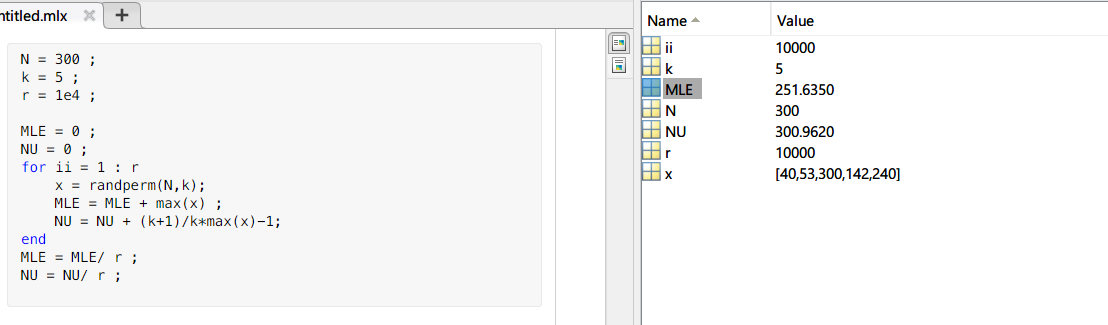
\includegraphics[width=15cm]{002.png}
  \caption{Figure2}\label{fg2}
\end{figure}
\end{center}



\end{document}
